\documentclass[11pt,border=10pt]{standalone}
\usepackage[T1]{fontenc}
\usepackage{lmodern}
\IfFileExists{Jost.sty}{\usepackage{Jost}}{}
\usepackage{tikz}
\usetikzlibrary{automata,positioning,arrows.meta,calc,decorations.pathmorphing}
\usepackage{xcolor}

\definecolor{teal}{HTML}{004D40}
\definecolor{coral}{HTML}{FF655D}
\definecolor{yellow}{HTML}{F1DB4B}
\definecolor{successgreen}{HTML}{2E7D32}
\definecolor{backoffred}{HTML}{C62828}

\begin{document}
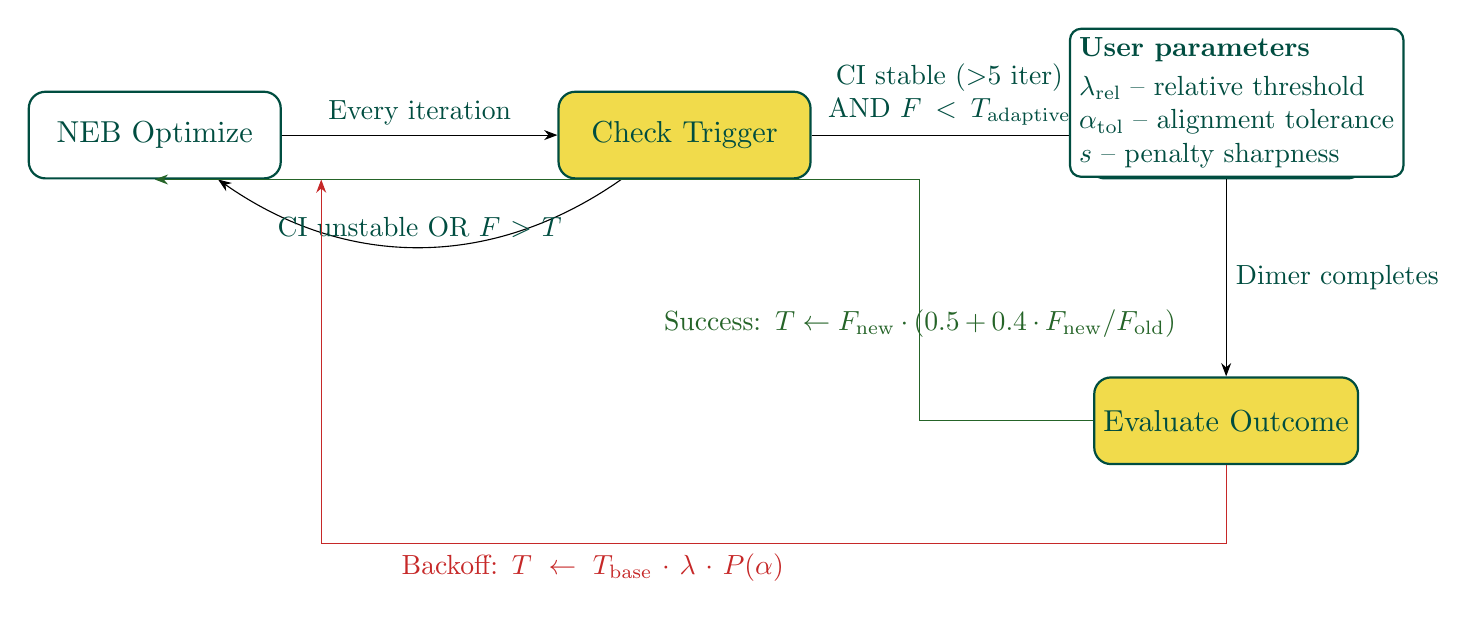
\begin{tikzpicture}[
    >=Stealth,
    every node/.style={font=\fontsize{11}{13}\selectfont},
    state/.style={
      rectangle, rounded corners=6pt,
      draw=teal, thick,
      minimum width=3.2cm, minimum height=1.1cm,
      text=teal, fill=white,
      align=center
    },
    decision/.style={
      rectangle, rounded corners=6pt,
      draw=teal, thick,
      minimum width=3.2cm, minimum height=1.1cm,
      fill=yellow, text=teal,
      align=center
    },
    highlight/.style={
      rectangle, rounded corners=6pt,
      draw=teal, thick,
      minimum width=3.2cm, minimum height=1.1cm,
      fill=coral, text=white,
      align=center
    },
    edgelabel/.style={font=\fontsize{10}{12}\selectfont, text=teal},
    every edge/.style={draw=teal, thick, ->},
  ]

  % Nodes
  \node[state]     (neb)   {NEB Optimize};
  \node[decision]  (check) [right=3.5cm of neb]  {Check Trigger};
  \node[highlight] (dimer) [right=3.5cm of check] {Run Dimer (MMF)};
  \node[decision]  (eval)  [below=2.5cm of dimer] {Evaluate Outcome};

  % Transitions
  \draw[->] (neb) -- node[edgelabel, above] {Every iteration} (check);

  % Loop back: CI unstable
  \draw[->] (check) to[bend left=35]
    node[edgelabel, above, align=center, text width=4cm]
      {CI unstable OR $F > T$}
    (neb);

  % Trigger fires
  \draw[->] (check) -- node[edgelabel, above, align=center, text width=4.2cm]
    {CI stable ($>$5 iter)\\AND $F < T_{\mathrm{adaptive}}$}
    (dimer);

  % Dimer completes
  \draw[->] (dimer) -- node[edgelabel, right] {Dimer completes} (eval);

  % Success path
  \draw[->, successgreen!80!black] (eval.west) -- ++(-2.2,0) |- (neb.south)
    node[edgelabel, pos=0.25, below, align=center, text=successgreen!80!black,
         text width=6.5cm]
      {Success: $T \leftarrow F_{\mathrm{new}} \cdot (0.5 + 0.4 \cdot F_{\mathrm{new}}/F_{\mathrm{old}})$};

  % Backoff path
  \draw[->, backoffred] (eval.south) -- ++(0,-1.0)
    -| ([xshift=0.5cm]neb.south east)
    node[edgelabel, pos=0.35, below, align=center, text=backoffred,
         text width=6.5cm]
      {Backoff: $T \leftarrow T_{\mathrm{base}} \cdot \lambda \cdot P(\alpha)$};

  % Parameter box
  \node[draw=teal, thick, rounded corners=4pt, fill=white,
        text=teal, font=\fontsize{10}{12}\selectfont,
        align=left, anchor=north east]
    at ([xshift=0.5cm, yshift=0.8cm]dimer.north east)
    {%
      \textbf{User parameters}\\[2pt]
      $\lambda_{\mathrm{rel}}$ -- relative threshold\\
      $\alpha_{\mathrm{tol}}$ -- alignment tolerance\\
      $s$ -- penalty sharpness%
    };

\end{tikzpicture}
\end{document}
